\chapter{Testes Hipóteses}

Um \textbf{teste de hipóteses} é um procedimento que usa estatística amostral para testar uma alegação sobre o valor de um parâmetro populacional. A finalidade de testes de hipóteses é avaliar uma afirmação sobre os valores de parâmetros populacionais. Uma alegação sobre um parâmetro populacional é chamada de \textbf{hipótese estatística}. Para testar uma hipótese estatística, você deve estabelecer cuidadosamente um par de hipóteses – uma representa uma alegação e a outra, seu complemento.

A \textbf{Hipótese Nula} (denotada por \(H_0\)) é uma hipótese estatística que contém uma
afirmativa de igualdade e deve escrever como \( = , \leq , \geq \). A \textbf{Hipótese Alternativa} (denotada por \(H_a\)) é o complemento da hipótese nula. É uma afirmativa que deve ser verdadeira se \(H_0\) for falsa e contém uma afirmativa de desigualdade, tal como \(<, \neq, ou > \).

A figura \ref{fig:hipoteses-estatisticas} a seguir mostra a relação entre as afirmativas verbais possíveis sobre o parâmetro \(\mu\) e as hipóteses nula e alternativa correspondentes. Afirmativas semelhantes podem ser feitas para outros parâmetros populacionais, tais como p (proporção), \(\sigma\) (desvio padrão) ou \(\sigma^2\) (variância).

\begin{figure}[h]
	\center
	\caption{Hipóteses Estatísticas para \(\mu\)}	
	\label{fig:hipoteses-estatisticas}
	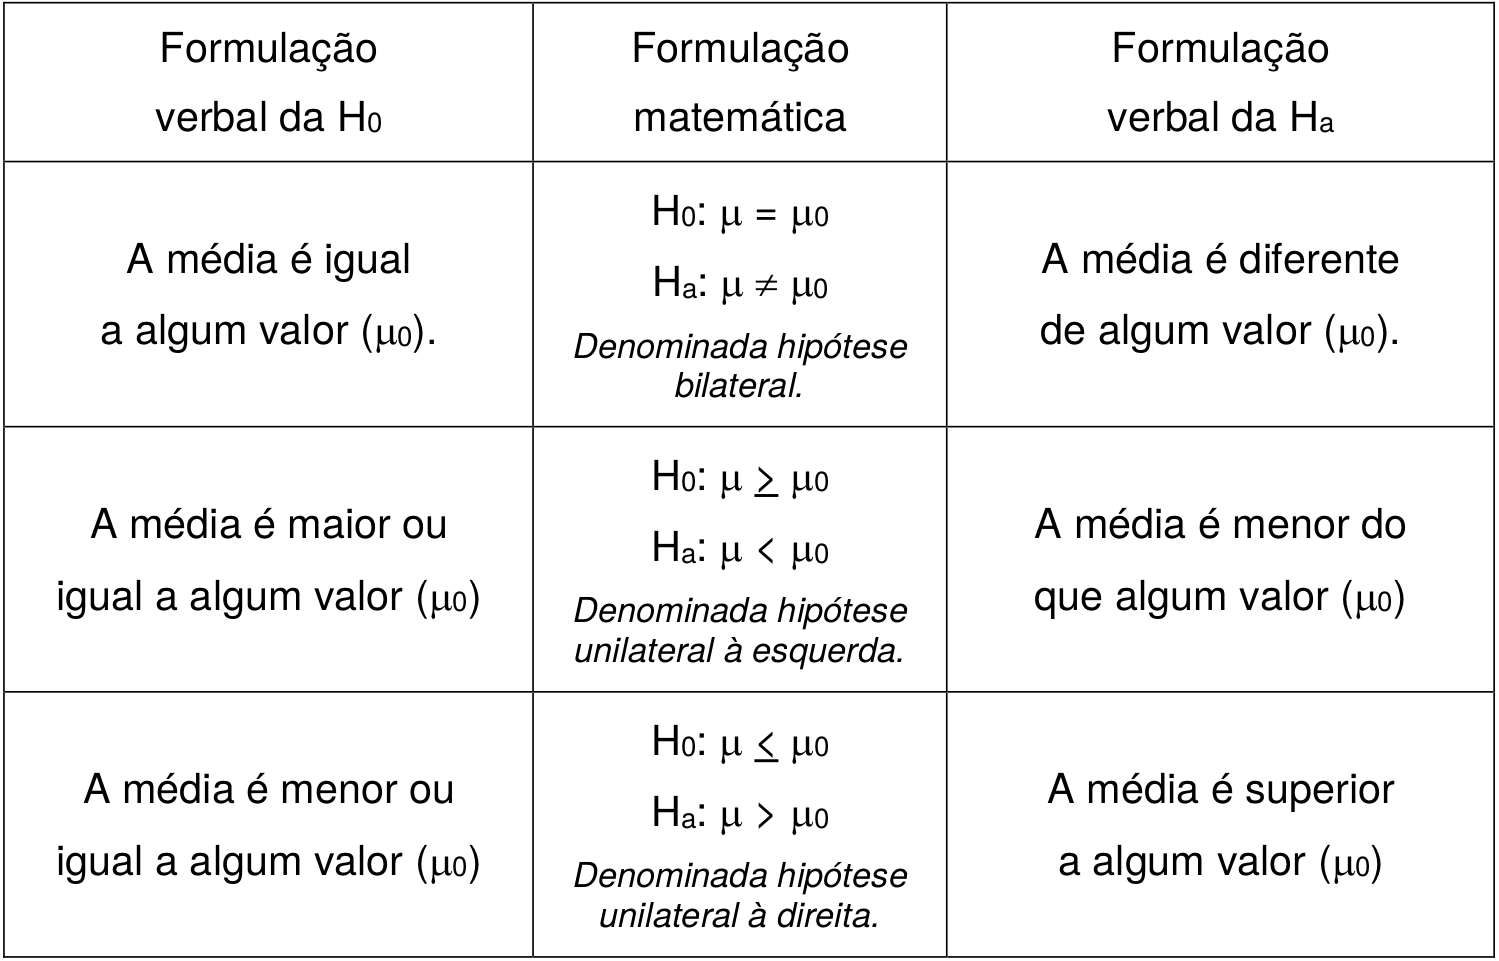
\includegraphics[scale=1.2]{testes-hipoteses/hipoteses-estatisticas.png}
\end{figure}

\section{Tipos de Erro e Nível de Significância}

Não importando qual das hipóteses representa a alegação, você começará sempre um teste de hipóteses assumindo que a condição de igualdade na hipótese nula é verdadeira. Assim, quando realizar um teste de hipóteses, você deve tomar uma de duas decisões: rejeitar a hipótese nula ou aceitar a hipótese nula.

Uma vez que sua decisão baseia-se em informação incompleta (uma amostra em vez de toda a população), há sempre a possibilidade de se tomar a decisão errada. A figura \ref{fig:resultados-teste-hipoteses} mostra os quatro resultados possíveis de um teste de hipóteses.

\begin{figure}[h]
	\center
	\caption{Possíveis Resultados para um Teste de Hipóteses}	
	\label{fig:resultados-teste-hipoteses}
	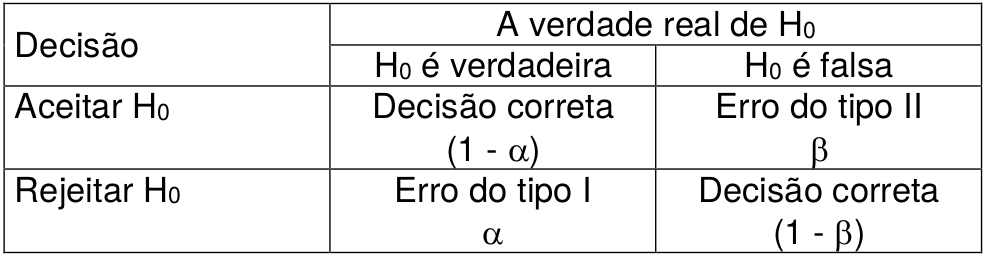
\includegraphics[scale=1.7]{testes-hipoteses/resultados-teste-hipoteses.png}
\end{figure}

O \textbf{nível de significância (\(\alpha\))} de um teste é a probabilidade de uma hipótese nula ser rejeitada, quando verdadeira. Uma das etapas de nosso processo de teste de hipóteses envolve a escolha do nível de significância. Pode-se mostrar, matematicamente, que \(\alpha\), \(\beta\) e o tamanho (n) da amostra estão todos inter-relacionados, de forma que, escolhidos quaisquer dois deles, o terceiro está
automaticamente determinado. Valem as seguintes considerações de ordem prática:
\begin{alineas}
\item Para \(\alpha\) fixo, um aumento do tamanho n da amostra ocasiona uma redução
de \(\beta\); isto é, uma amostra maior reduz a chance de cometermos o erro de aceitar a hipótese nula quando ela é falsa.
\item Para um tamanho n, fixo, de amostra, uma diminuição de \(\alpha\) acarreta um aumento de \(\beta\); reciprocamente, um aumento de \(\alpha\) acarreta uma diminuição de \(\beta\).
\item Para reduzir \(\alpha\) e \(\beta\), devemos aumentar o tamanho da amostra.
\end{alineas}

\section{Estatística de Teste, Região Crítica e Valor Crítico}

A \textbf{estatística de teste} é uma estatística amostral, ou um valor baseado nos dados
amostrais. Utiliza-se uma estatística de teste para tomar uma decisão sobre a rejeição ou não da hipótese nula. A \textbf{região crítica} é o conjunto de todos os valores da estatística de teste que levam à rejeição da hipótese nula. O \textbf{valor crítico} é o valor, ou valores, que separa(m) a região crítica dos valores da estatística de teste que não levam à rejeição da hipótese nula. Os valores críticos dependem da natureza da hipótese nula, da distribuição amostral principal, e do nível de significância.

O método clássico de testes de hipóteses  utilizando região crítica constiste nos seguintes passos:
\begin{alineas}
\item Identificar a hipótese nula (contém a condição de igualdade) e a hipótese alternativa (complementar);
\item Escolher o nível de significância com base na gravidade do erro tipo I. São
muito comuns os valores 0,05 e 0,01;
\item Identificar o teste a ser utilizado;
\item Determinar a estatística de teste;
\item Determinar o(s) valor(es) crítico(s) e a região crítica;
\item Rejeitar \(H_0\) se a estatística de teste está na região crítica. Aceitar \(H_0\) se a estatística de teste não está na região crítica;
\item Formular uma conclusão que descreva a conseqüência prática dos dados e dos cálculos.
\end{alineas}

\section{Teste z para uma Amostra (\(\sigma\) conhecido)}

O teste z é utilizado em testes de hipóteses para a média quando valor do desvio padrão (\(\sigma\) é conhecido. Identificadas as hipóteses estatísticas (\(H_0\) e \(H_a\)) e definido o nível de significância (\(\alpha\)), podemos proceder ao cálculo da estatística de teste utilizando a fórmula a seguir.

\[\beq{ z_{teste} = \frac{\hat{x}-\mu_0}{\frac{\sigma}{\sqrt{n}}} } \]

Onde \(\mu_0\) representa o valor da média que está sendo testado, \(\sigma\) representa o desvio padrão populacional, n é o tamanho da amostra e \(\hat{x}\) é a média da amostra.

\subsection{Com base no nível de significância (\(\alpha\))}

\begin{itemize}
	\item Fornecidos: \(\alpha\), \(\mu_0\), \(\hat{x}\) e \(\sigma\)
	\item Aplicar a fórmula de \(z_{teste}\)
	\item Encontrar \(z_{\alpha}\) considerando:
	\begin{itemize}
		\item O sinal de \(z_{teste}\)
		\item O tipo de hipótese (unilateral à esquerda, à direita ou bilateral)
		\item A interpretação da probabilidade na Tabela da Normal Reduzida
	\end{itemize}
\end{itemize}		
	
\subsection{Com base no valor \(p\)}

\begin{itemize}
	\item Fornecidos: \(\alpha\), \(\mu_0\), \(\hat{x}\) e \(\sigma\)
	\item Aplicar a fórmula de \(z_{teste}\)
	\item Encontrar \(p\) considerando:
	\begin{itemize}
		\item O sinal de \(z_{teste}\)
		\item O tipo de hipótese: unilateral à esquerda, à direita ou bilateral 
		\item \(p\) acompanha \(H_a\)
		\item A interpretação da probabilidade na Tabela da Normal Reduzida
		\item Interpretação: comparar \(p\) e \(\alpha\). Se \(p \leq \alpha\) a hipótese nula deve ser rejeitada.
	\end{itemize}
\end{itemize}		

\subsection{Com base no intervalo de confiança}

A correspondência direta entre um intervalo de confiança e um teste de hipótese pode ser feita somente quando o teste é bilateral.

\section{Teste t para uma amostra (\(\sigma\) desconhecido)}

O teste t é utilizado em testes de hipóteses para a média quando valor do desvio padrão (\(\sigma\) é desconhecido. Nesse caso, deve utilizar o desvio padrão amostral (\(s\)) e a distribuição t-Student. Identificadas as hipóteses estatísticas (\(H_0\) e \(H_a\)) e definido o nível de significância (\(\alpha\)), podemos proceder ao cálculo da estatística de teste utilizando a fórmula a seguir.

\[\beq{ t_{teste} = \frac{\hat{x}-\mu_0}{\frac{s}{\sqrt{n}}} } \]

Onde \(\mu_0\) representa o valor da média que está sendo testado, \(s\) representa o desvio padrão amostral, n é o tamanho da amostra e \(\hat{x}\) é a média da amostra.

O valor crítico é obtido na tabela t-Student, a partir do número de graus de liberdade (n -1). Após determinar o número de graus de liberdade (na linha da tabela) e localizar, na coluna, o valor correspondente à área da cauda que se deseja obter, o valor crítico será o valor que corresponde ao cruzamento da linha e da coluna que foram determinados. Lembrando que se um valor crítico está localizado na cauda esquerda, devemos considerá-lo negativo.

\subsection{Com base no valor \(p\)}

\begin{itemize}
	\item Fornecidos: \(\alpha\)\footnote{Lembrar de que \(\alpha\) é uma probabilidade.}, \(\mu_0\), \(\hat{x}\) e \(s\)
	\item Aplicar a fórmula para encontrar o \(t_{teste}\)
	\item Encontrar \(p\) considerando:
	\begin{itemize}
		\item O sinal de \(t_{teste}\)
		\item O tipo de hipótese (unilateral à esquerda, à direita ou bilateral)
		\item A interpretação da probabilidade na Tabela da t-Student:
			\begin{itemize}
				\item Buscar o valor mais próximo do \(t_{teste}\) na linha do grau de liberdade
				\item O valor de \(p\) é o cabeçalho correspondente ao valor encontrado na tabela t-Student
			\end{itemize}
		\item Interpretação: comparar \(p\) e \(\alpha\). Se \(p \leq \alpha\) a hipótese nula deve ser rejeitada.
	\end{itemize}
\end{itemize}

\subsection{Com base no intervalo de confiança}

A correspondência direta entre um intervalo de confiança e um teste de hipótese pode ser feita somente quando o teste é bilateral.

\section{Teste de Hipóteses para a Proporção}

Os testes de hipóteses para proporções são adequados quando os dados sob análise consistem de contagens ou frequências de itens. A finalidade de tais testes é avaliar afirmações sobre a proporção (ou percentagem) de uma população.

Suposições:
\begin{itemize}
	\item Condições para um experimento binomial
	\item Condições \(n.p_0\geq5\) e \(n.(1-p_0)\geq5\)
\end{itemize}

Estatística de teste:

 \[\beq{ z_{teste} = \frac{\hat{p}-p_0}{\sqrt{\frac{p_0(1-p_0)}{n}}} }\]
 
Em muitos aspectos, o teste de hipóteses para uma proporção se assemelha grandemente ao teste z, principalmente pelo fato de que utilizam a mesma distribuição de probabilidades. Dessa forma, a região crítica, o valor crítico e o valor p para o teste de proporção são obtidos exatamente da mesma maneira que o teste z para uma média.

\section{Teste z para Comparação de Duas Proporções}

Um teste z de duas amostras é usado para testar a diferença entre duas proporções \(p_1\) e \(p_2\) quando uma amostra é selecionada aleatoriamente de cada população.

Condições:
\begin{itemize}
	\item As amostras devem ser selecionadas aleatoriamente.
	\item As amostras devem ser independentes.
	\item As amostras devem ser grandes o suficiente para usar uma distribuição normal de amostragem (\( n_1p_1 > 5, n_1q_1 > 5, n_2p_2 > 5 \) e \( n_2q_2 > 5. \)).
\end{itemize}

Notação:
\begin{itemize}
	\item \(n_1 = \) tamanho da 1\textsuperscript{a} amostra
	\item \(n_2 = \) tamanho da 2\textsuperscript{a} amostra
	\item \(x_1 = \) número de sucessos da 1\textsuperscript{a} amostra	
	\item \(x_2 = \) número de sucessos da 2\textsuperscript{a} amostra		
	\item \(\hat{p}_1 = \) proporção de sucessos da 1\textsuperscript{a} amostra	
	\item \(\hat{p}_2 = \) proporção de sucessos da 2\textsuperscript{a} amostra		
\end{itemize}

\subsection{Abordagem pelo valor p}

\begin{verbatim}
	Estratégia sugerida: Geogebra 
\end{verbatim}

Estatística de teste:

\[\beq{ z = \frac{\hat{p_1}-\hat{p_2}}{\sqrt{\frac{\bar{p}(1-\bar{p})}{n_1}+\frac{\bar{p}(1-\bar{p})}{n_2}} }}\]

onde, a estimativa ponderada para \(p_1\) e \(p_2\) pode ser obtida por:

\[\bar{p}=\frac{n_1\hat{p}_1 + n_2\hat{p}_2}{n_1+n_2}\]

Conclusão:
\begin{itemize}
	\item Se \(p \leq \alpha\), rejeitarmos \(H_0\).
	\item Se \(p > \alpha\), aceitarmos \(H_0\).
\end{itemize}

\subsection{Abordagem pelo intervalo de confiança}

\begin{verbatim}
	Estratégia sugerida: Python 
\end{verbatim}

\[\beq{ (\hat{p}_1-\hat{p}_2) \pm z_{\frac{1-\alpha}{2}} \sqrt{\frac{\bar{p}(1-\bar{p})}{n_1}+\frac{\bar{p}(1-\bar{p})}{n_2}} }\]

Interpretação:

\begin{itemize}
	\item se o intervalo contém 0 (zero) há indícios de que as duas proporções são iguais, caso contrário, se o intervalo não contém 0 (zero) pode-se concluir com \( 100(1-\alpha)\% \) de confiança que as duas proporções são diferentes.
		\item Se os limites do intervalo do confiança apresentam sinal negativo (-) pode-se dizer que a proporção da 2\textsuperscript{a} amostra é maior do que a proporção da 1\textsuperscript{a} amostra.
	\item Ao contrário, se os limites do intervalo apresentarem sinal positivo (+) conclui-se que a proporção da 1\textsuperscript{a} amostra é maior que a proporção da 2\textsuperscript{a} amostra.
\end{itemize}

\section{Teste t para Comparação de Duas Médias (Amostras Pareadas)}

Uma amostra pareada corresponde ao levantamento de dados da mesma amostra em duas situações nas quais tenha interferido algum fator cujo efeito deseja-se avaliar (Ex.: Comparar o peso de um grupo de pessoas antes e depois de passarem por uma dieta rigorosa).

Suposições:
\begin{itemize}
	\item Deve-se escolher de maneira aleatória duas amostras dependentes de duas populações.
	\item Ambas as populações devem ter distribuição Normal. Se elas se afastam radicalmente da distribuição Normal, devemos utilizar os métodos não-paramétricos.
\end{itemize}

\subsection{Abordagem pelo valor p}

\begin{verbatim}
	Estratégia sugerida: Python 
\end{verbatim}

\begin{alineas}
	\item Estabeleça o nível de significância (\(\alpha\)) a ser adotado. Se \(\alpha\) não for fornecido, adotar o valor padrão 0.05.
	\item Estabelecer as hipóteses:
		\begin{alineas}
			\item \(H_0\): Médias pareadas iguais (antes e depois): \(\mu_1 = \mu_2\)
			\item \(H_1\): Médias pareadas significativamente diferentes\footnote{Nesse material, trataremos somente a hipótese bilateral.}: \(\mu_1 \neq \mu_2\)
		\end{alineas}
	\item Encontrar o valor \(\bar{d}\) que é a média das diferenças \(d_i\): 

	\[\beq{ \bar{d} = \frac{\sum{d_i}}{n} }\]

	\item Calcular o desvio padrão \(s_d\) das diferenças \(d_i\):

	\[\beq{ s_d = \sqrt{\frac{n(\sum{d_i^2})(\sum{d_i})^2}{n(n-1)}} }\]	
	
	\item Calcular a estatística de teste \(T_p\):
	
	\[\beq{ T_p = \frac{\bar{d}}{ \frac{s_d}{\sqrt{n}}} }\]
	
	\item Calcular o valor \textbf{p}: \(p = 2 \times P(t>|T_p|) \), com n-1 graus de liberdade.

	\item Conclusão:
		\begin{alineas}
			\item Se p \(\leq\) nível de significância (\(\alpha\)), então há indícios para rejeitarmos \(H_0\).
			\item Se p > nível de significância (\(\alpha\)), então há evidências suficientes para aceitarmos \(H_0\).
		\end{alineas}

\subsection{Abordagem pelo intervalo de confiança}

\begin{verbatim}
	Estratégia sugerida: Python 
\end{verbatim}

\[\beq{ \bar{d} \pm t_{n-1;\frac{\alpha}{2}} \times \frac{s_d}{\sqrt{n}}  }\]
	
\end{alineas}

\section{Teste F para Comparação de Duas Variâncias (Bilateral)}

\begin{verbatim}
	Estratégia sugerida: Python 
\end{verbatim}

Esse teste é, muitas vezes, usado em conexão com o teste t-Sudent para duas médias (amostras
independentes), em que é necessário verificar a homocedasticidade (igualdade) ou
heterocedasticidade (diferença) das variâncias. Para duas amostras aleatórias e independentes, de tamanhos \(n_1\) e \(n_2\), retiradas de duas populações normais com variâncias \(\sigma_1^2\) e
\(\sigma_2^2\). Desejamos testar a hipótese bilateral: 

\[H_0: \sigma_1^2 = \sigma_2^2\]

\[H_a: \sigma_1^2 \neq \sigma_2^2\]

Estatística de teste:

\[ F = \frac{\sigma_1^2}{\sigma_2^2} \]

Valores críticos:

\[\beq{ F_L = \frac{1}{F_{n_2-1;n1-1;\frac{\alpha}{2}}} }\]

\[\beq{ F_R = F_{n_1-1;n2-1;\frac{\alpha}{2}} }\]

Os valores \( F_{n_2-1;n1-1;\frac{\alpha}{2}} \) e \(F_{n_1-1;n2-1;\frac{\alpha}{2}}\) são encontrados na  tabela F. Para um nível de significância \(\alpha\):
\begin{itemize}
	\item Rejeitar \(H_0\) se \(F < F_L\) ou se \(F>F_R\)
	\item Caso contrário, não rejeitamos \(H_0\)
\end{itemize} 